\section{Introduction}

Additive manufacturing (or 3D Printing) is an emerging technology, in which different objects are printed in layers having a 3D model as a reference. This technology made rapid prototyping faster and enabled the creation of custom-shaped objects. However this process is not always perfect and printing errors are to be expected.Modern 3D printers come with vision systems that can capture the printing process, so this defect detection task can be posed from the perspective of a computer vision task. \\
The patterns of the defects can be observed and a classical detection algorithm e.g. Template Matching can be tuned to detect a specific type of pattern. The shortcoming of this approach is the lack of generalization. Therefore, the algorithm requires manual tuning each time a new pattern appears or the dataset is changed. A more modern approach to this modern is to use convolutional neural networks. \\
In the current setup, the 3D printer uses binder jetting technology. This type of printing uses two materials: a powder based material and a binding agent. The printer head moves along the printing surface and deposits alternating layers of sand and binding agent in accordance to a model \cite{binder_jetting}. This technology stands out by being able to print very large objects. \\
\begin{figure}[!h]
  \centering
  \captionsetup{justification=centering,margin=2cm}
  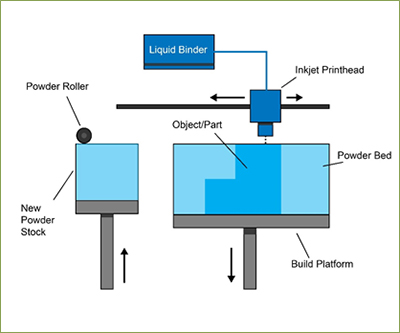
\includegraphics[width=0.5\linewidth]{images/introduction/binderjetting}
  \caption{A sketch of a 3D printer}
  \label{intro:printer}
\end{figure}
In this thesis a YOLO-based neural network solution is proposed and explored for this automatization procedure.  \\

\subsection{Considered Dataset}
As mentioned in the previous paragraphs, a 3D printer contains a camera to track the printing process. This camera is usually positioned directly above the printing surface and can capture each layer individually. In the presented images, the printing defects are vertical scratches, which are also visible on grayscale images as dark lines. In figure \ref{fig:layer_00325_marked_cropped} the printing defects are highlighted with some bounding boxes. \\

\begin{figure}[!h]
  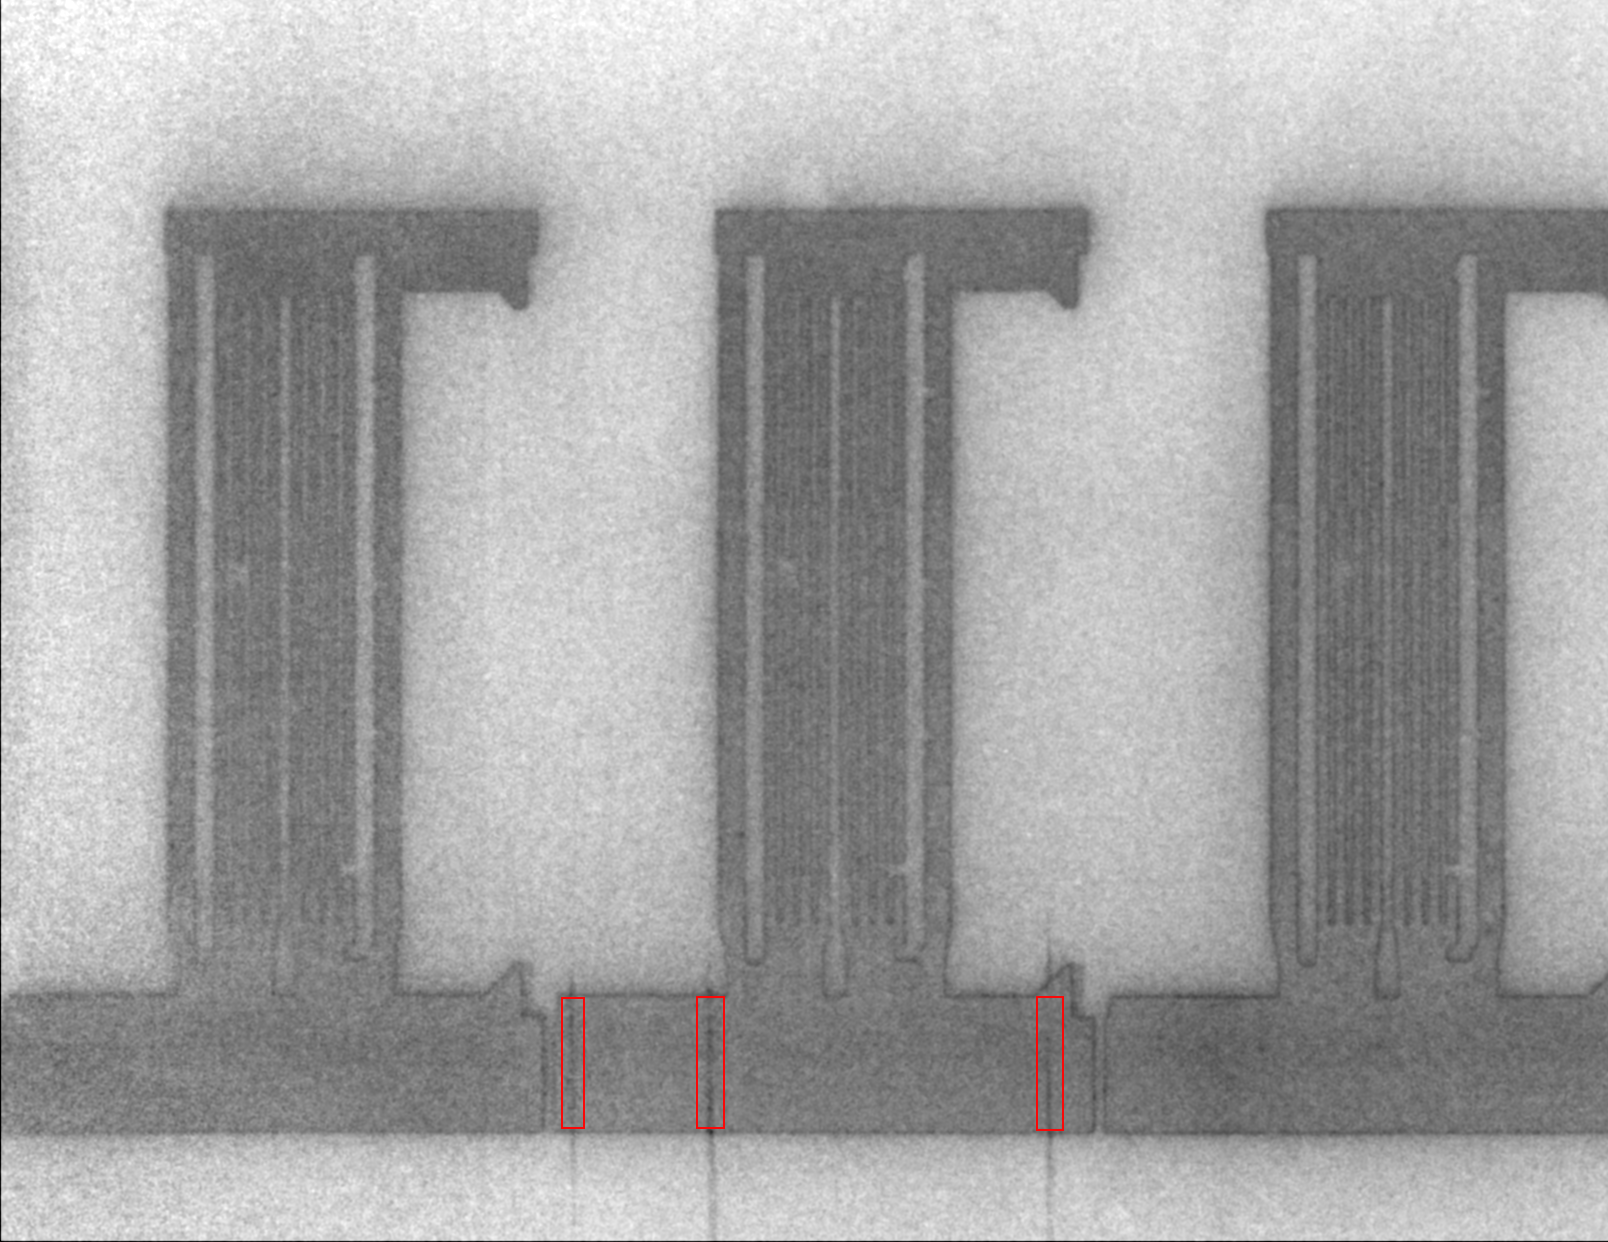
\includegraphics[width=0.65\textwidth]{images/layer_00325_marked_cropped}
  \centering
  \caption{}
  \label{fig:layer_00325_marked_cropped}
\end{figure}

The image of the layer seen in figure \ref{fig:layer_00325_marked_cropped} has actually been through a pre-processing step called camera calibration. This process calculates a parameter called camera matrix, which can be used to correct the distortion of images. This process works by capturing a known pattern with the camera and then through more complex algorithms, the distortion between the captured pattern and the actual pattern can be parametrized with the camera matrix. The most common calibration pattern is a chessboard, because it is easy to identify it's corners. However, in order to calibrate the camera of the 3D printer a large pattern is required (about 180x100 cm), but for practicality a layer with a grid of crosses is printed and then captured. A captured calibration pattern can be seen in figure \ref{intro:calibration} and a strong radial distortion can be observed. \\

\begin{figure}[!h]
  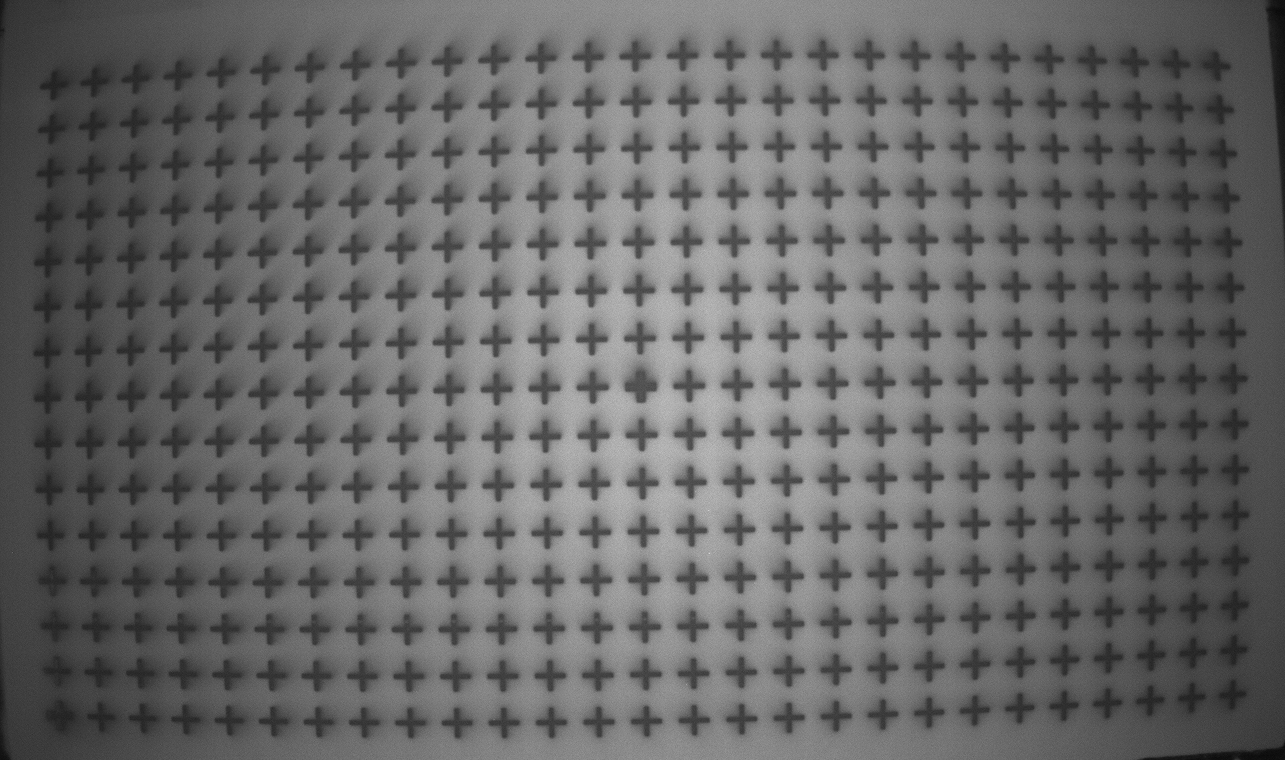
\includegraphics[width=0.65\textwidth]{images/introduction/calibration_pattern}
  \centering
  \caption{The captured calibration pattern}
  \label{intro:calibration}
\end{figure}

The 3D models used by the printer can be actually represented as an image for each layer. In this case, the information provided would be to print or not to print at a specific square 1x1 mm. This information can be easily encoded with a 1800x1000 bitmask, in which the 1's mark the regions to be printed. The interesting part is that those bitmasks are actually the ideal image of each layer and it would be very helpful to integrate this knowledge in the training process. \\

\begin{figure}[!h]
\centering
\begin{subfigure}{.5\textwidth}
  \centering
  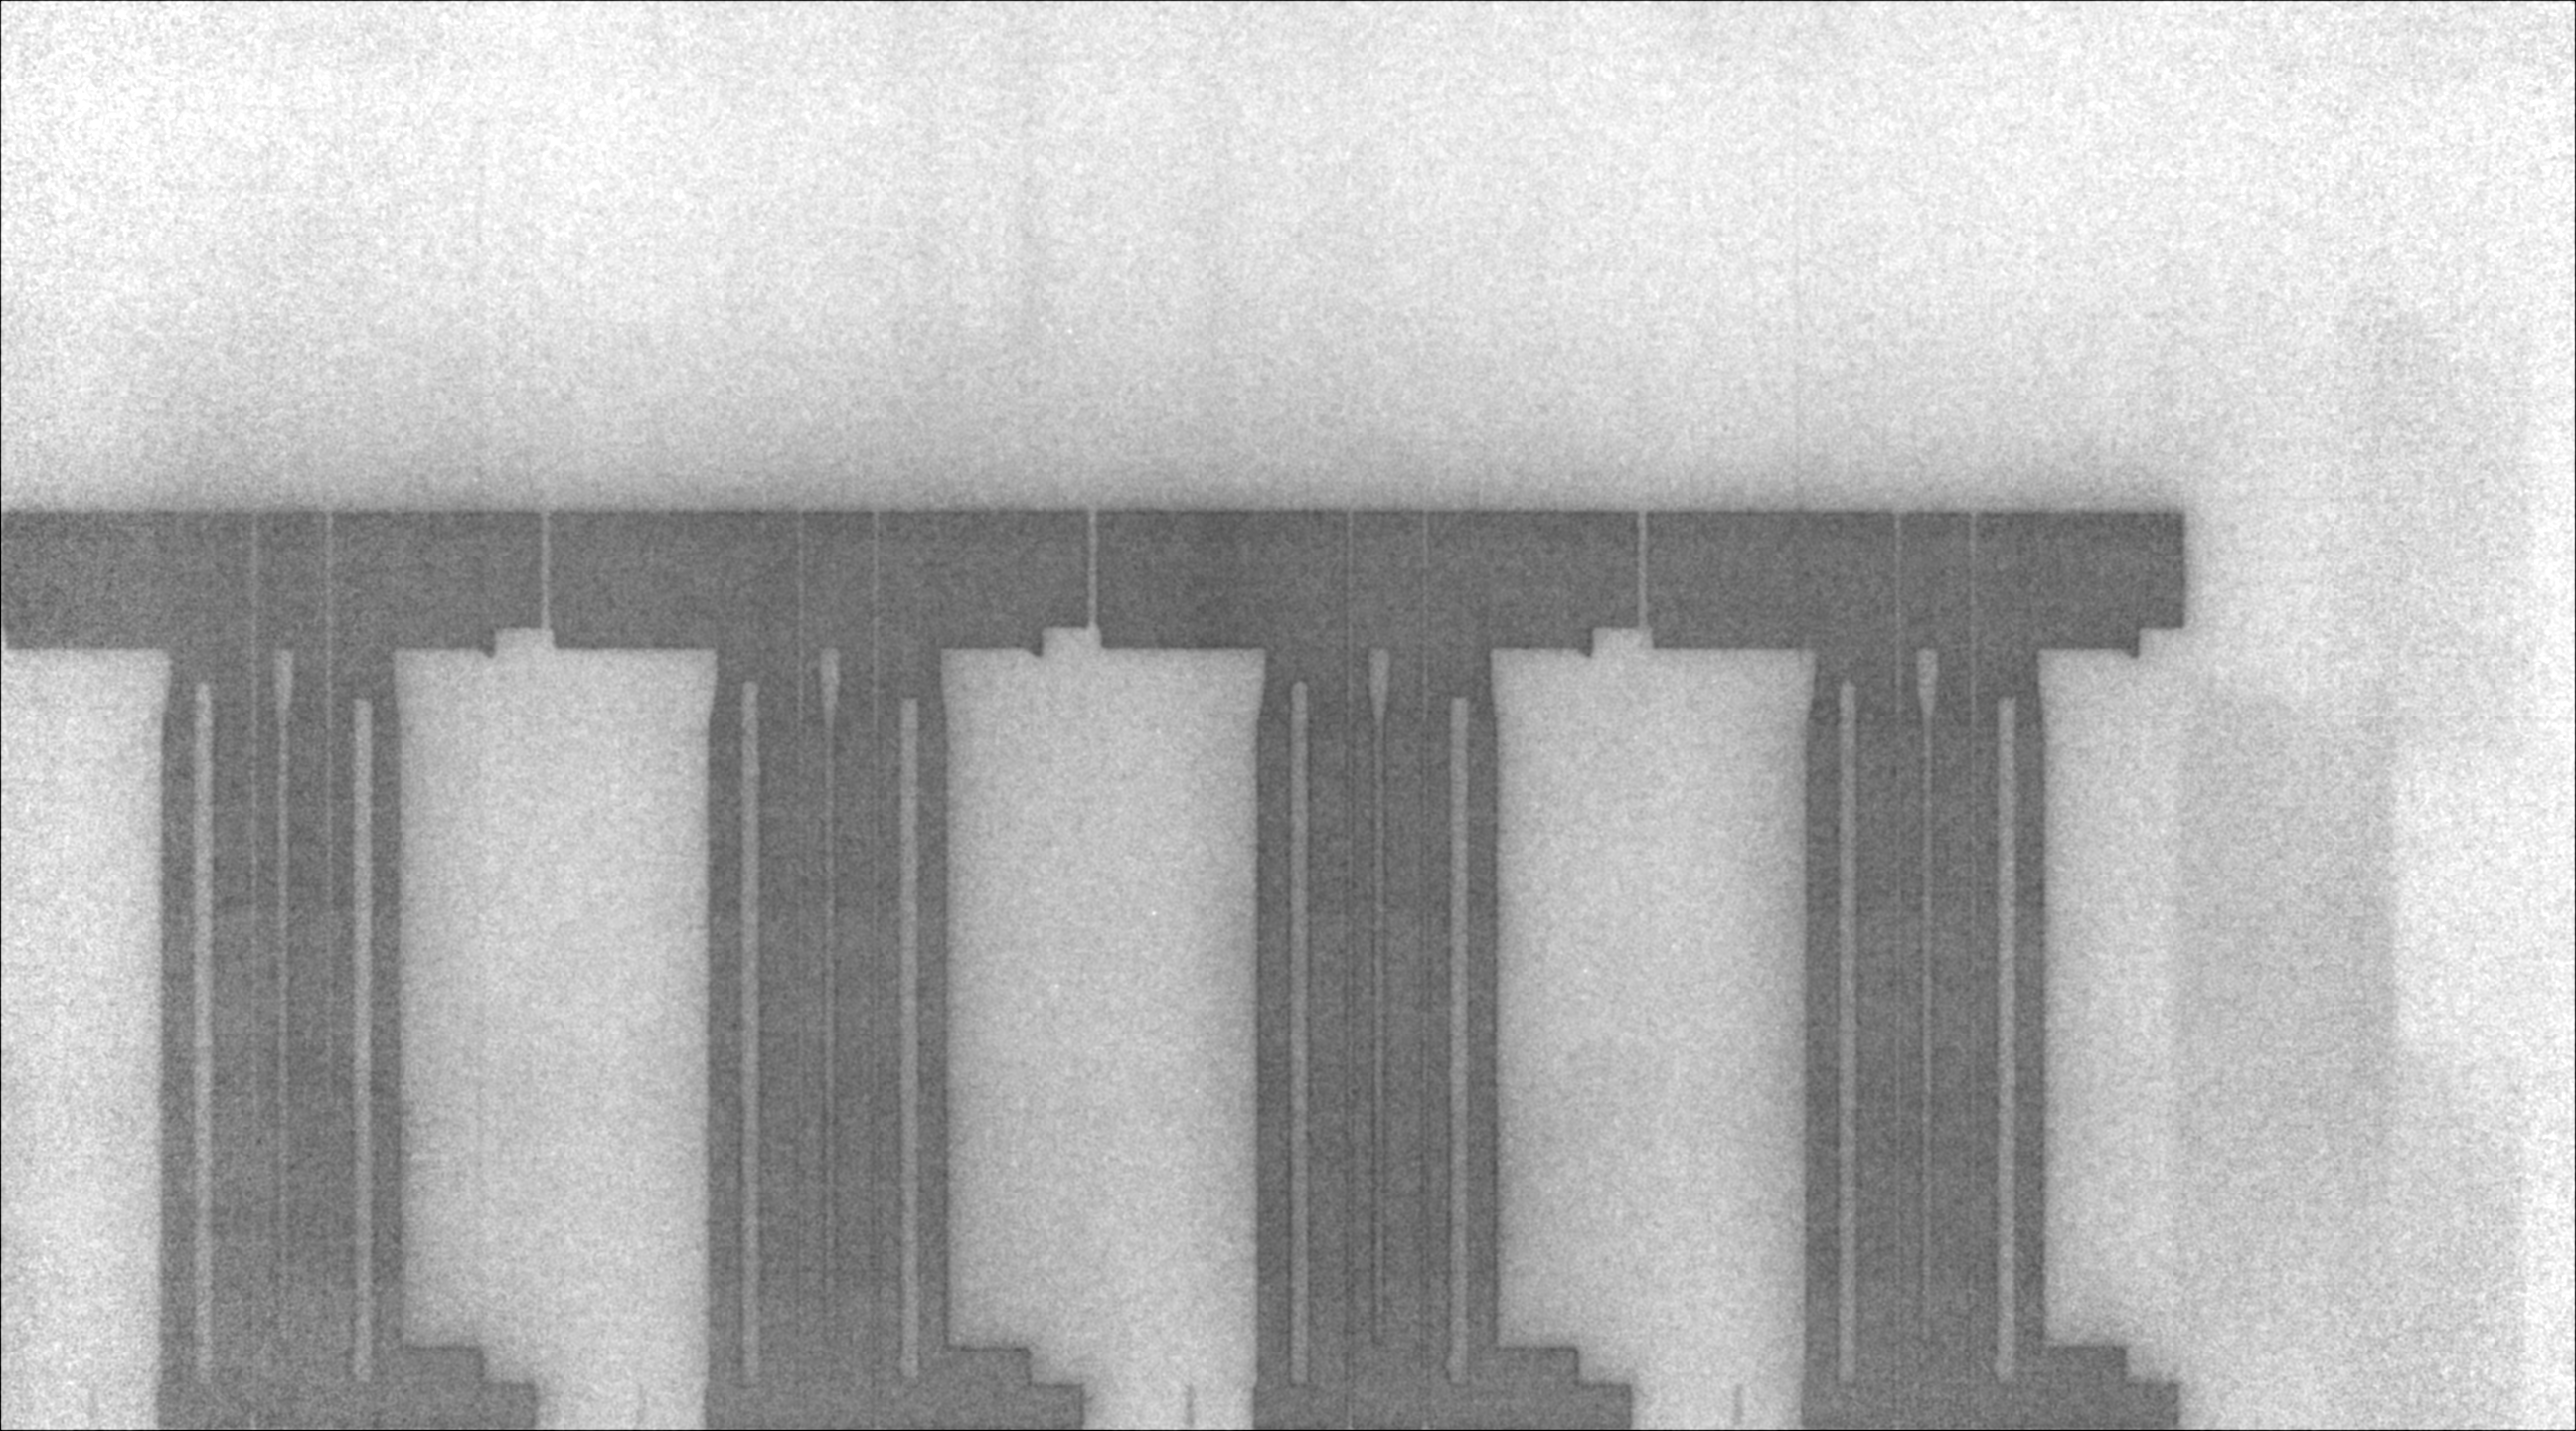
\includegraphics[width=.5\linewidth]{images/introduction/layer_00100}
  \caption{A layer image}
\end{subfigure}%
\begin{subfigure}{.5\textwidth}
  \centering
  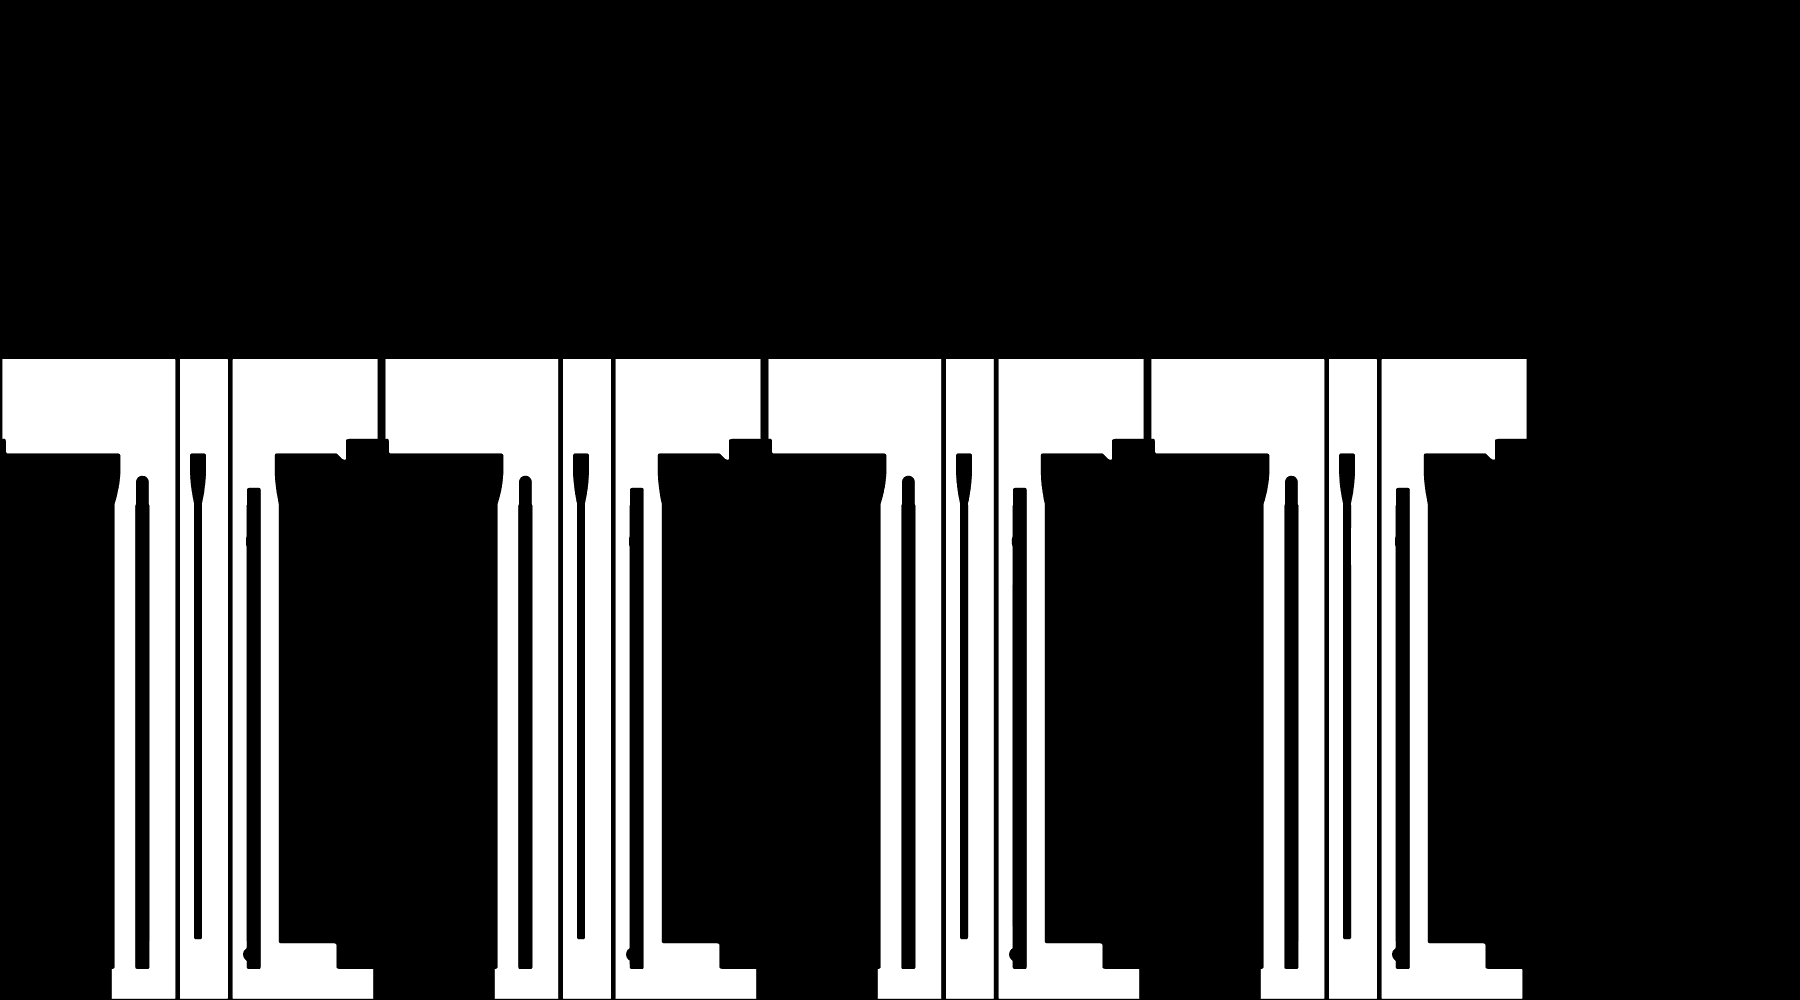
\includegraphics[width=.5\linewidth]{images/introduction/bitmask_00100}
  \caption{The bitmask}
\end{subfigure}
\caption{The printed layer and the corresponding bitmask used during the printing process.}
\label{intr:layer_example}
\end{figure}

This table should provide an overview of the dataset on hand:
\begin{table}[!h]
\centering
\begin{tabular}{ ||c|c||}
\hline
dataset property & value \\ [0.5ex]
\hline\hline
total images & 2295 \\
captured image resolution & 2592x1440 \\
bitmask resolution & 1800x1000 \\
captured image ratio & 1.8 \\
bitmask image ratio & 1.8 \\
images with scratchs & $\approx$ 300 \\
total scratches & $\approx$ 650 \\
\hline
\end{tabular}
\label{asdfsdfdf}
\caption{Stats about the current dataset.}
\end{table}


\subsection{Object Detection (With Neural Networks)}
There are a variety of techniques used to perform object detection. Initially, object detection was posed as a non-neural computer vision problem, but this required a constant and tedious manual tuning of parameters. In order to avoid this tuning, feature-based machine learning algorithms were developed e.g. Viola-Jones algorithm  \cite{viola_joines_paper}. In this way the parameter tuning was partially automatized, but it still required manual tuning like selecting the optimal Haar features for the Viola-Jones algorithm.
One step further in this direction was the introduction of deep-learning based methods, which use a neural network at heart. A trained neural network would be albe to detect objects with way less parameter tuning. The drawback is that a considerable amount of labeled data for training is now required, which mostly is manually labeled. Luckily, today there are many open source labeled datasets that easily contain hundreds of thounsands of images e.g. ImageNet Dataset \cite{imagenet_site}, OpenImages Dataset \cite{openimages_site}. \\
Because of the already labeled datasets, the manual labor for deep-learning based methods was greatly reduced and the focus shifted towards those kind of methods, leading to the creation of many innovative models. One distinction among deep-learning based methods, regarding data labeling, is that the objects can be labeled with bounding boxes or segmentation masks. Models that use bounding boxes tend to train and predict faster, while models with segmentation masks will have the benefit of optimizing predictions to a pixel level. Another consideration would be that, if manual labeling is required, drawing bounding boxes is easier and less error prone than drawing an outline for segmentation masks. \\

\begin{figure}[!h]
\centering
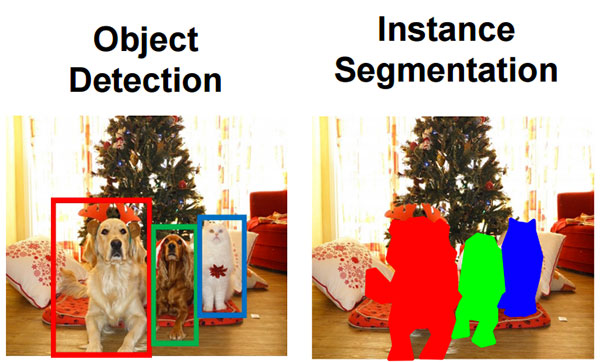
\includegraphics[width=0.65\textwidth]{images/bbs_vs_seg}
\caption{Labeling methods: on the left bounding boxes, on the right segmentation masks}
\end{figure}

Regarding the architecture of neural networks, the detection process may have one or two stages. In a single stage network the prediction is made directly from the extracted features of the image, while in a two stage network the network proposes some regions in the first stage and in the second stage the proposed regions are classified. Initially, single stage detectors predicted faster and could be used for real-time detections, but where performing poorer than two-stage detectors. Conversely, two-stage detectors were not optimal for real-time detection, but were more precise. This rule of thumb got overwritten with the release of You Only Look Once object detector (YOLO).

\begin{figure}[!h]
\centering
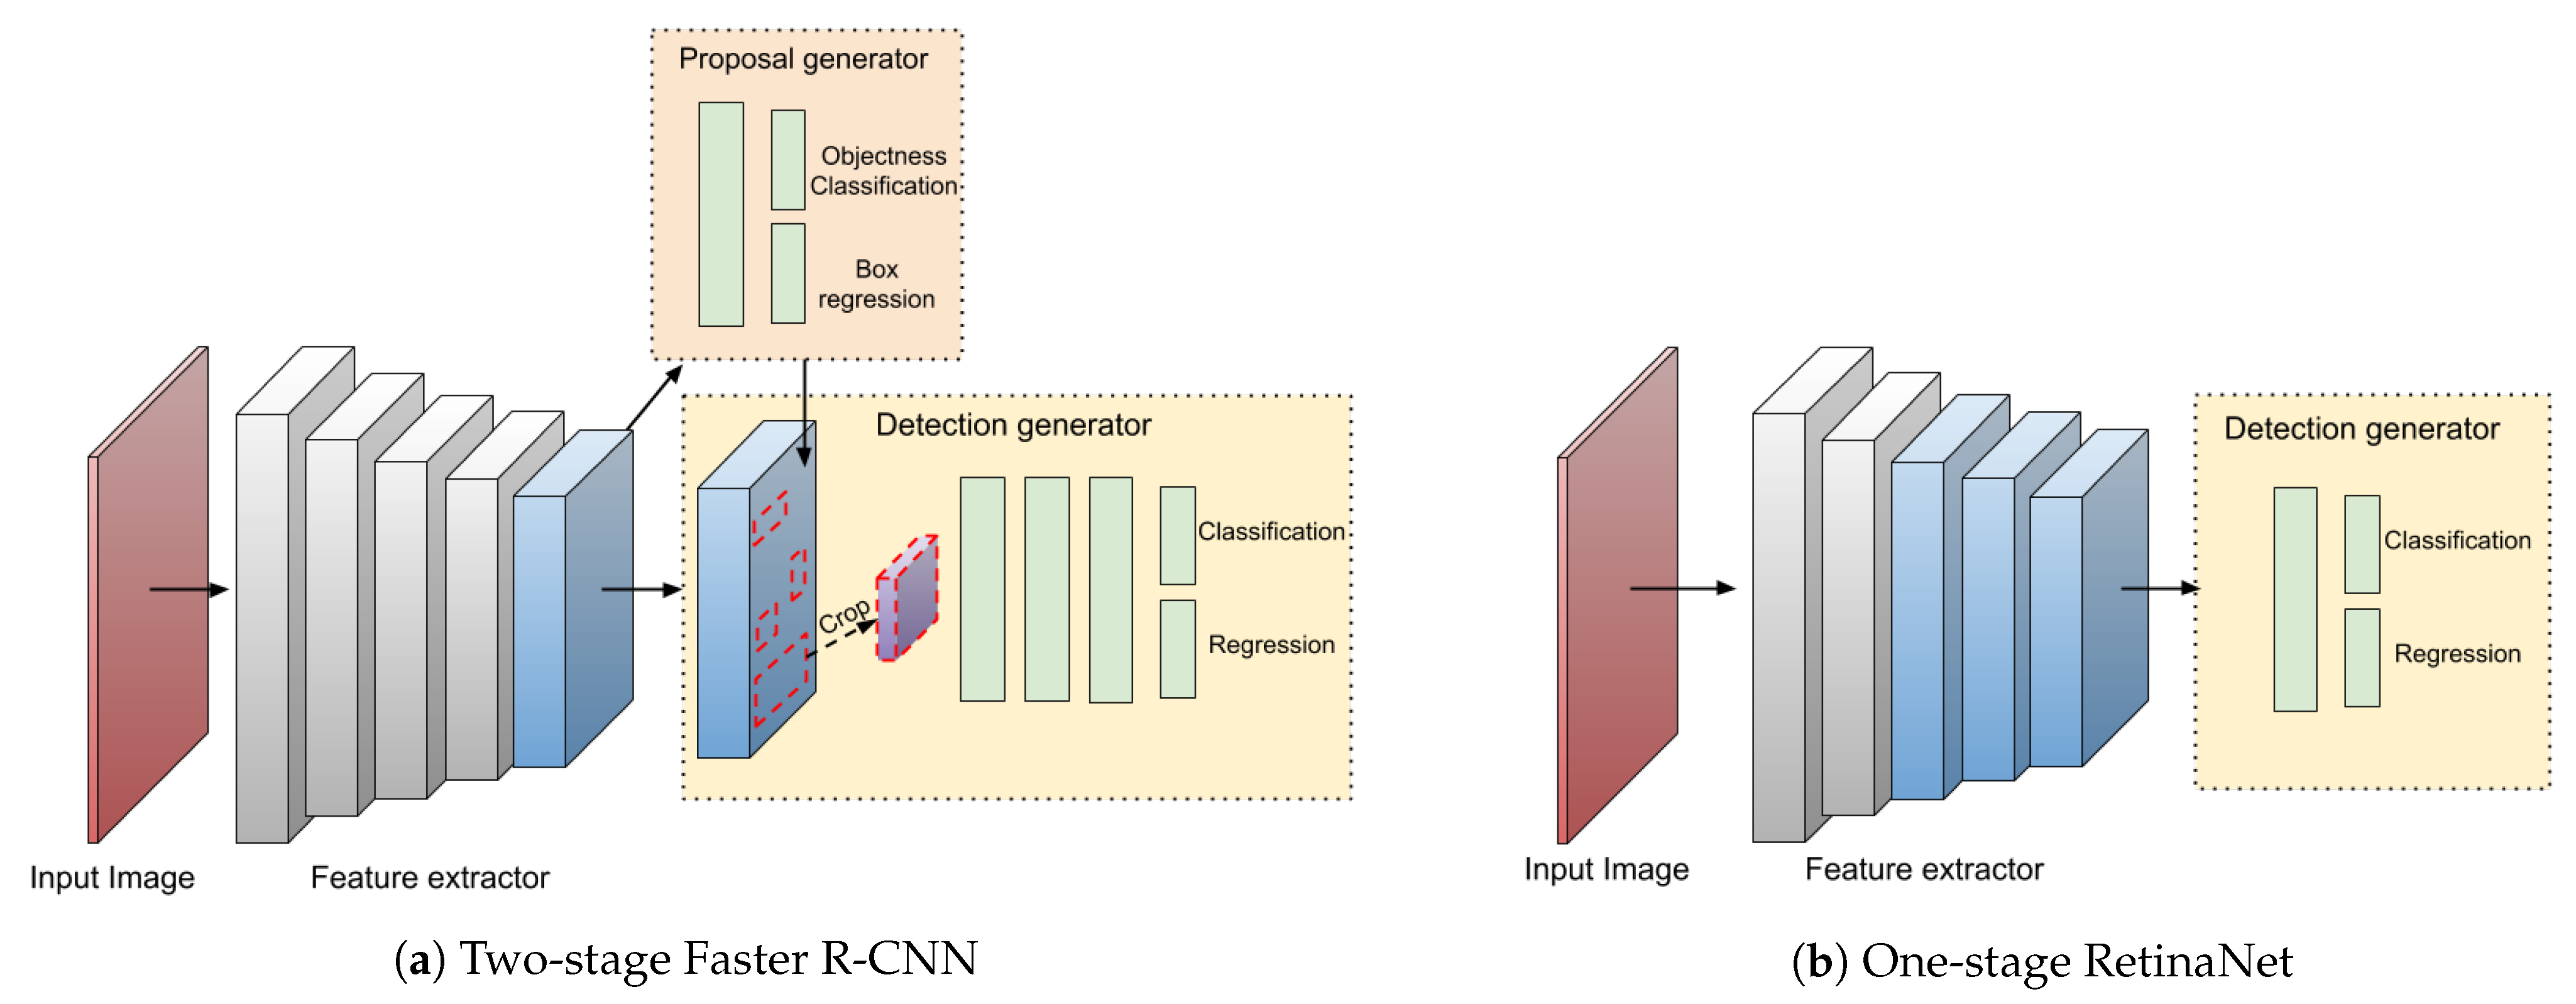
\includegraphics[width=0.75\textwidth]{images/single_stage_vs_two_stage}
\caption{Comparing stage types of object detectors.}
\end{figure}



The first YOLO object detector, now known as YOLOv1 \cite{yolov1_paper}, got a lot of attention for outperforming the then state-of-the-art object detectors such as DPM \cite{dpm_paper}, Fast R-CNN \cite{fast_rcnn_paper} and Faster R-CNN \cite{faster_rcnn_paper}. Also the simplicity of YOLO was quite refreshing for using only 24 convolutional layers and 2 fully connected layers only, unlike the sophisticated R-CNN based architectures. \\
Even if in some very deep model variations of Fast and Faster R-CNN the mean average precision (mAP) was slightly better,the FPS counter would take a massive hit e.g. 0.5 FPS only for Fast R-CNN. \\


\begin{table}
  \centering
    \begin{tabular}{ ||c|c|c|c||}
    \hline
    Detector & real-time? & mAP & FPS\\ [0.5ex]
    \hline\hline
    100Hz DPM & yes & 16.0 & 100 \\
    30Hz DPM & yes & 26.0 & 30 \\
    Fast YOLOv1 & yes & 52.7 & 155 \\
    YOLOv1 & yes & 63.4 & 45 \\
    Fastest DPM & no & 30.4 & 15 \\
    R-CNN Minus R & yes & 53.5 & 6 \\
    Fast R-CNN & yes & 70.0 & 0.5 \\
    Faster R-CNN VGG-16 & yes & 73.2 & 7 \\
    Faster R-CNN ZF & yes & 62.1 & 18 \\
    YOLO VGG-16 & yes & 66.4 & 21 \\
    \hline
    \end{tabular}
  \label{intro:yolov1_comp_table}
  \caption{YOLOv1 compared to then state-of-the-art models \cite{yolov1_paper}}
\end{table}

This first successful initial release of YOLO was a launch pad for development of subsequent YOLO versions, so that a new class of object detectors was born. This class of architecture contains 3 main components: backbone, neck and head.
The backbone has the role to extract features from the image, while the neck tries to aggregate the features from different stages from the backbone. In the end the head does the prediction. Usually the backbone has a quite simple build like ResNet-101 and Darknet-53 \cite{yolov3_paper}.For feature aggregation SPP \cite{spp_paper} and FPN \cite{fpn_paper} are a popular choice . \\
Later on, different research groups developed their own YOLO-based object detectors and non-canonical versions like YOLOv5 \cite{yolov5_git} and YOLOR \cite{yolor_paper} were created. With this many releases from different research groups, simply taking the latest YOLO version was not a viable choice anymore and for this thesis multiple versions have been tests.\\

\subsection{Main Challenges} \label{intro:challenges}
This sections provides an overview of the main challenges faced during the development and research of the YOLO-based object detector. The main challenge can be usually divided in smaller, more specific sub-challenges, which will be discussed in depth in the next chapter. In no particular order of importance, the main challenges are:

\textbf{Small dataset:}
As seen in section \ref{intro:dataset_sizes}, the images of the printed 3D layers are grayscale images and the target objects are some long thin scratches. This is in contrast with the open datasets that contain RGB images with 80 different objects, which do not even closely resemble a scratch. As a consequence, only the small dataset at hand of about 2300 images can be used for training. The situation gets even worse after discovering that only a fraction of the images contain scratches. \\
\begin{figure}[!h]
\centering
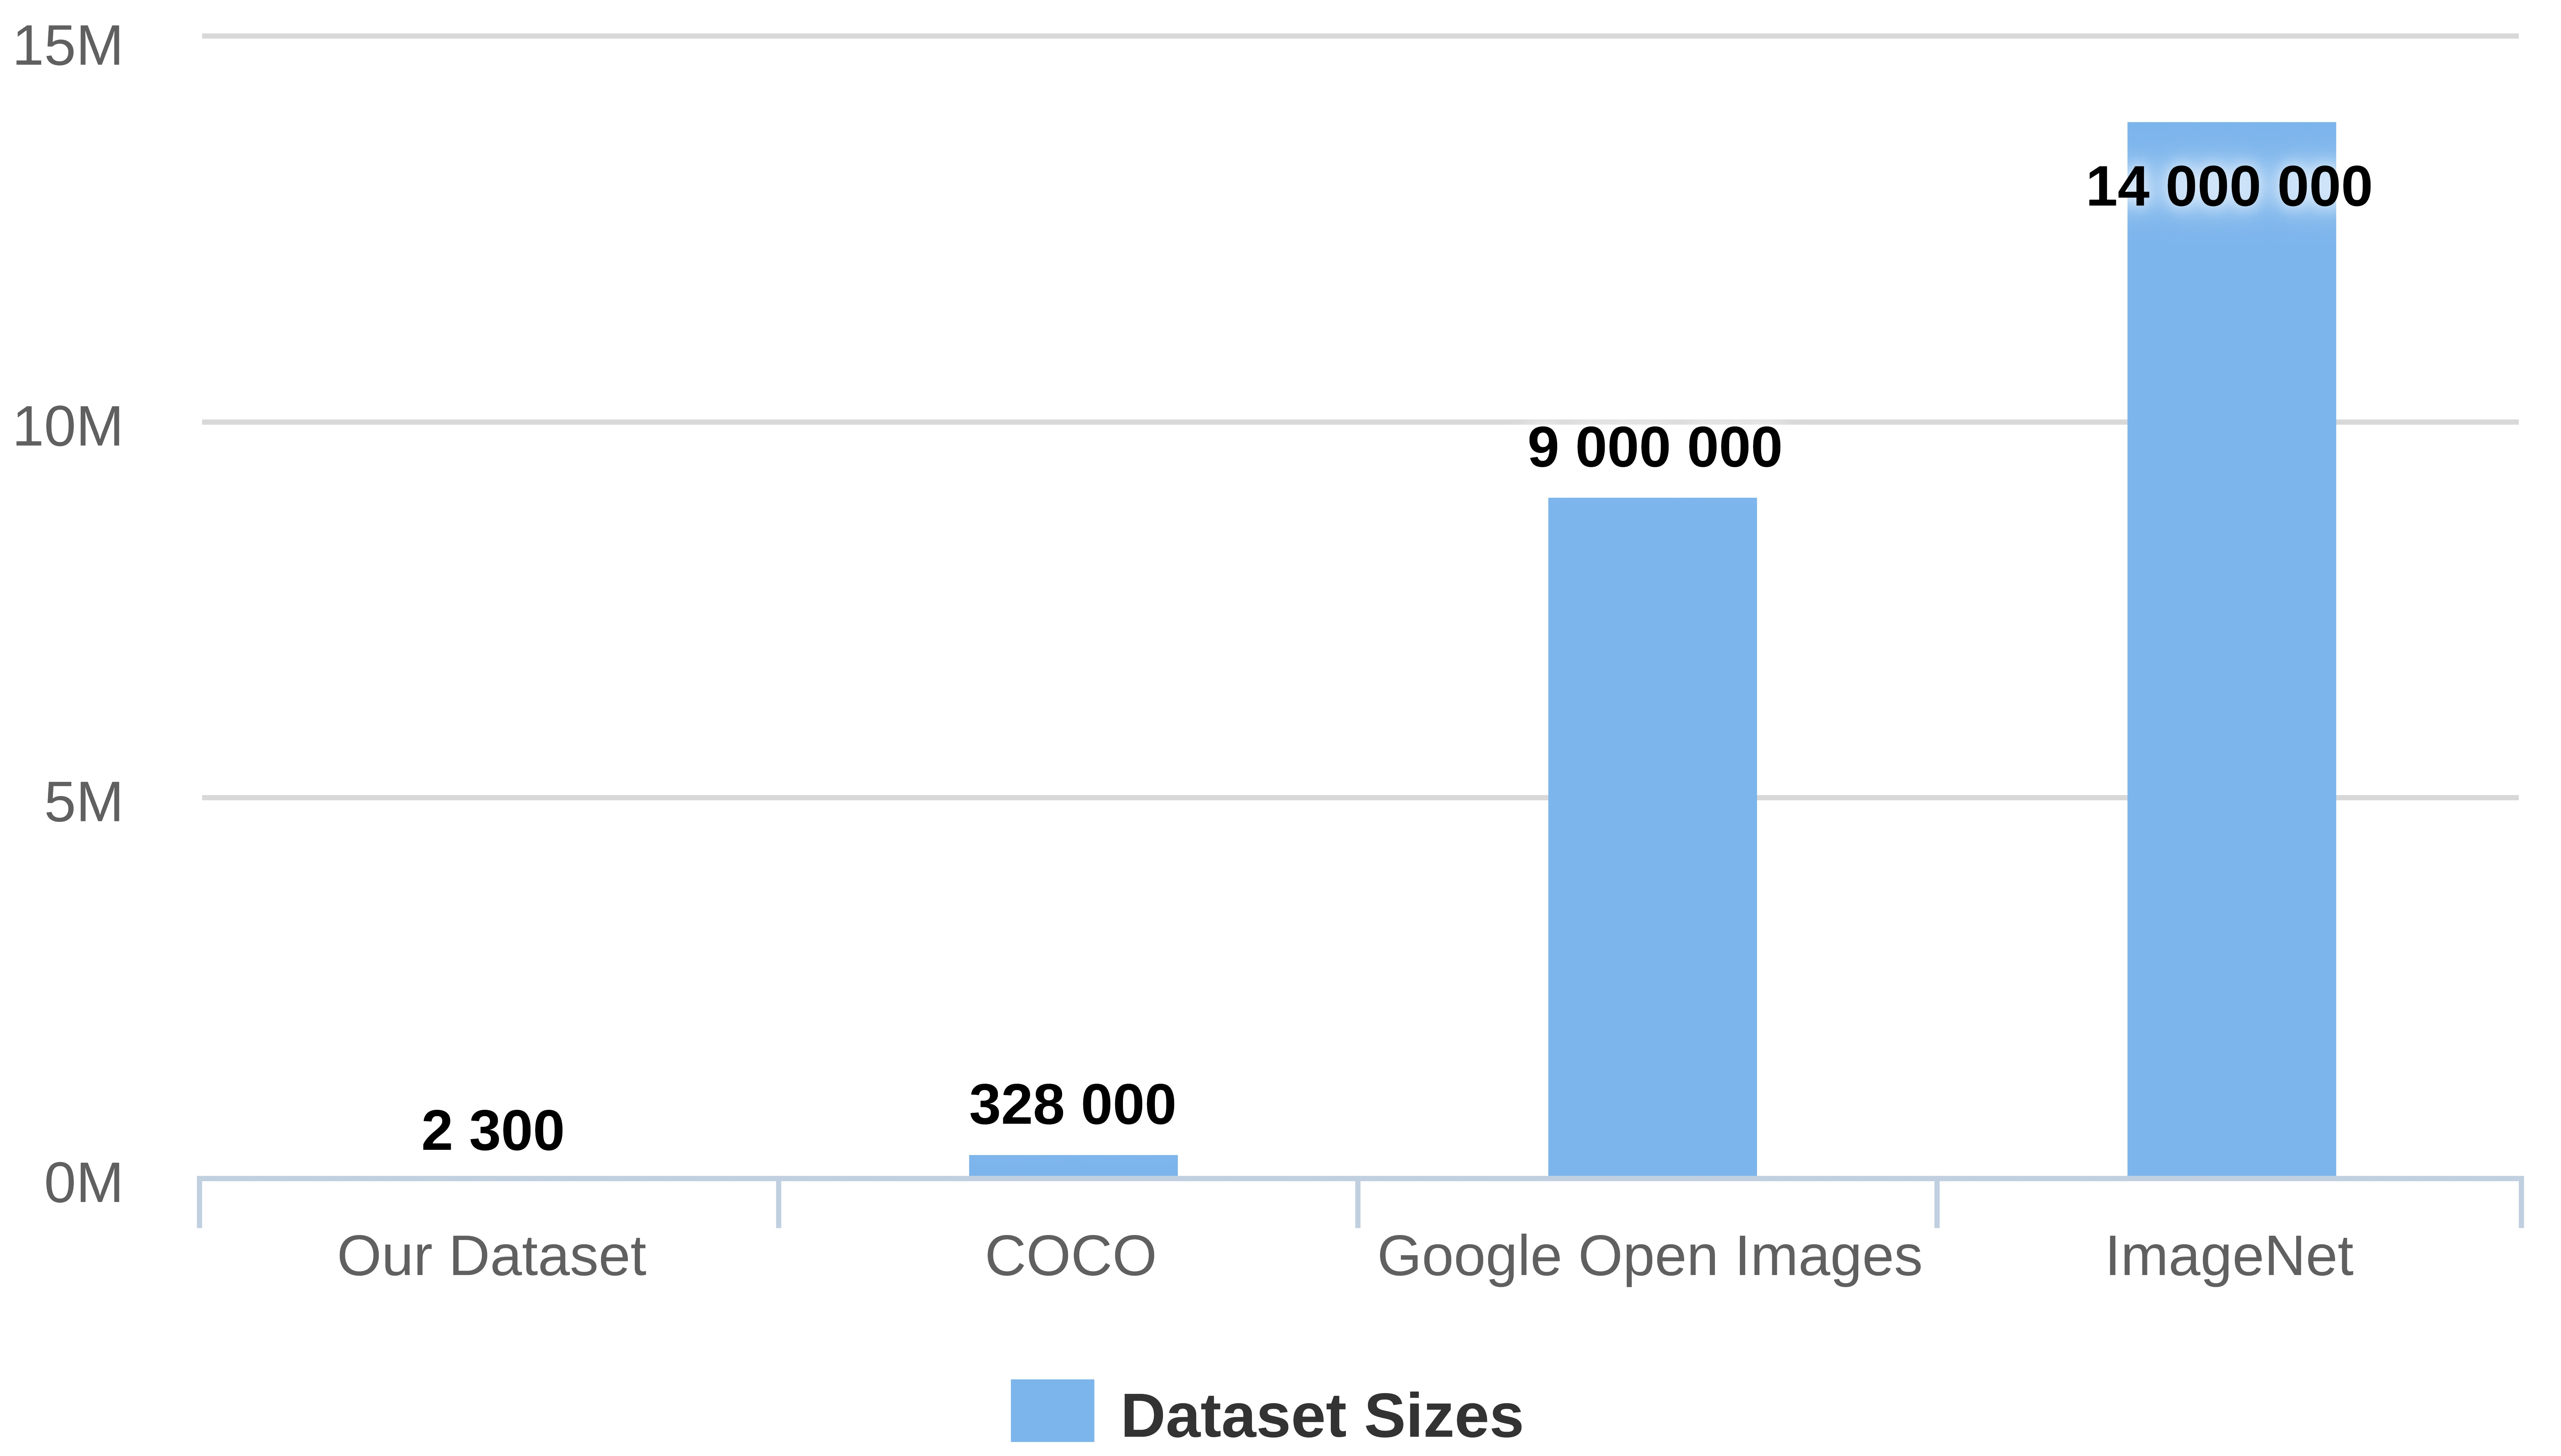
\includegraphics[width=0.4\columnwidth]{images/introduction/dataset_sizes}
\caption{The dataset on hand does not compare with the huge open datasets.}
\label{intro:dataset_sizes}
\end{figure}
A fortunate thing is that the scratches can fit very good in bounding boxes and no extra precision will be provided by the more tedious, time-consuming segmentation masks. This leads to the next point of labeling. \\



\textbf{Identifying relevant scratches:}
% alternative:  consistency of the labels
The scratches present in the dataset are sometimes very faded and annotating those scratches leads to an overly sensitive model. From a practical point of view, those scratches might not even affect the actual printed object. Therefore, only prominent and deep scratches need to be marked. \\
This is easier said than done, because humans have problems separating the weak scratches from strong scratches. This separation task is just an alternative version of Sorites Paradox actually. In figure \ref{intro:original_scratch_fades}, a gradient from stronger scratches to weaker ones can be seen. How can one determine an objective threshold between the stronger and weaker scratches? \\
Also being inconsistent with the annotation e.g. first images contain weaker scratches than the final images, is another problem. This inconsistency would only "confuse" the model.

\begin{figure}[!h]
\centering
\captionsetup{justification=centering,margin=2cm}

\includegraphics[width=\columnwidth]{images/introduction/original_scratch_fades}
\caption{A "gradient" of scratches. Which scratches are strong enough to be used for training?}
\label{intro:original_scratch_fades}
\end{figure}

The objectiveness and consistency are some key aspects in this situation, so some kind of metric is needed to ensure this.\\
In the usual open datasets, the objects are not in a transitory state from barely visible to visible, which makes in this point of view the dataset on hand more unique. \\
In the table below some relevant statistics about the dataset are presented:
\begin{center}
\begin{tabular}{ ||c|c|| }
\hline
property & value \\ [0.5ex]
\hline\hline
% total images & 2295 \\
% images with scratches & $\approx$ 300 \\
total scratches & $\approx$ 650 \\
scratch average length & 138 px \\
scratch median length & 117 px \\
scratch min length & 24 px \\
scratch max length & 630 px \\
scratch length std. deviation & 104 \\
% image size & $2592 \times 1440$ \\
% bitmask size & $1800 \times 1000$ \\

\hline
\end{tabular}
\end{center}


\textbf{Domain Knowledge Integration:}
As seen in figure \ref{intro:double_edge}, two close edges might look like a scratch, but the bitmask can be used to clarify the situation. This exact process of comparing the layer image with the respective bitmask is the motivation of including also the bitmask for training and inference. The problem is that most models take exactly one image and a file with labels as input and now a bitmask needs to be included somehow.\\

\begin{figure}[!h]
\centering
\begin{subfigure}{.5\textwidth}
  \centering
  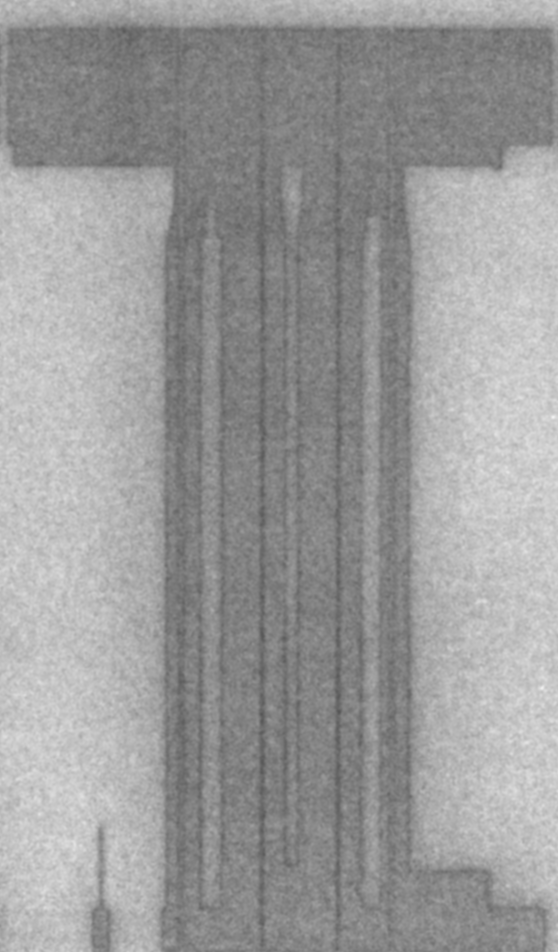
\includegraphics[width=.4\linewidth]{images/introduction/bitmask_integration/layer_00091}
  \caption{A crop from a layer image}
\end{subfigure}%
\begin{subfigure}{.5\textwidth}
  \centering
  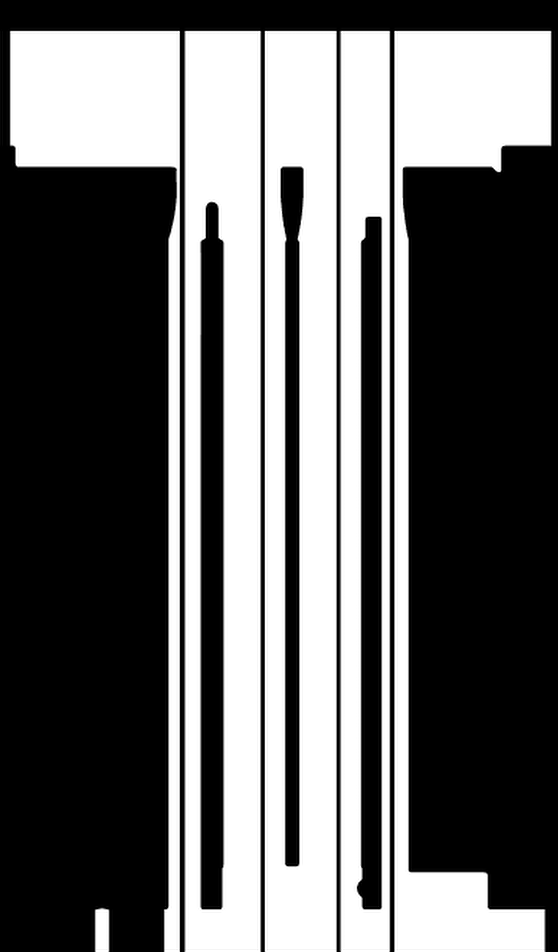
\includegraphics[width=.4\linewidth]{images/introduction/bitmask_integration/bitmask_00091}
  \caption{The corresponding bitmask}
\end{subfigure}
\caption{Two closely positioned edges generate can look like a scratch, but the bitmask clearly shows that there is actually no scratch.}
\label{intro:double_edge}
\end{figure}

Another problem is that small artifacts from previous layers can be visible in the current layer, which again might look like a scratch. This means that looking at previous bitmasks is also helpful during labeling. Therefore, the model needs to be aware also of previous bitmasks. Now the problem from the previous paragraph evolved into including multiple bitmasks. This situation can be seen in figure \ref{intro:image_artifacts} \\

\begin{figure}[!h]
\centering
\begin{subfigure}{.33\textwidth}
  \centering
  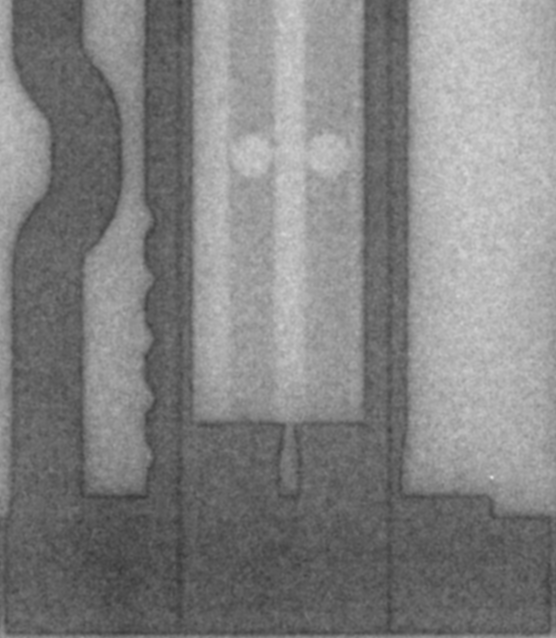
\includegraphics[width=.5\linewidth]{images/introduction/bitmask_integration/layer_00830}
  \caption{Layer image}
\end{subfigure}%
\begin{subfigure}{.33\textwidth}
  \centering
  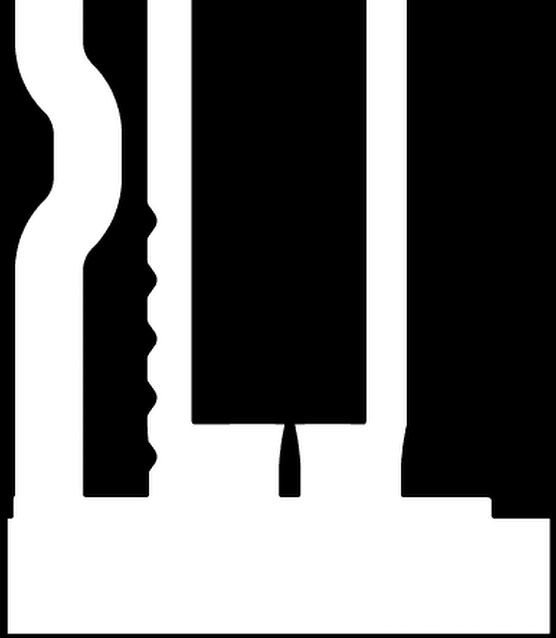
\includegraphics[width=.5\linewidth]{images/introduction/bitmask_integration/bitmask_00830}
  \caption{Current bitmask}
\end{subfigure}
\begin{subfigure}{.33\textwidth}
  \centering
  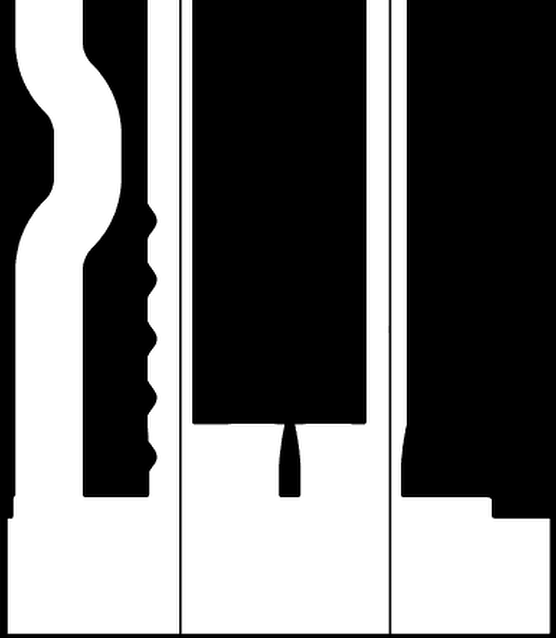
\includegraphics[width=.5\linewidth]{images/introduction/bitmask_integration/bitmask_00829}
  \caption{Previous bitmask}
\end{subfigure}
\caption{In the layer image dark lines that look like scratches are visible, but the current bitmask does not indicate the the presence of gap between two edges like in figure \ref{intro:double_edge}. However the previous bitmask shows where the dark lines from the layer image actually come from.}
\label{intro:image_artifacts}
\end{figure}

Other anomalies like dark spots from the an uneven oxidation are also possible. In some cases those spots have a thin and tall shape that also can be confusing to tell if it's a scratch. Such an example can be seen in figure \ref{intro:layer_oxidation}.


\begin{figure}[!h]
\centering
\begin{subfigure}{0.75\textwidth}
  \centering
  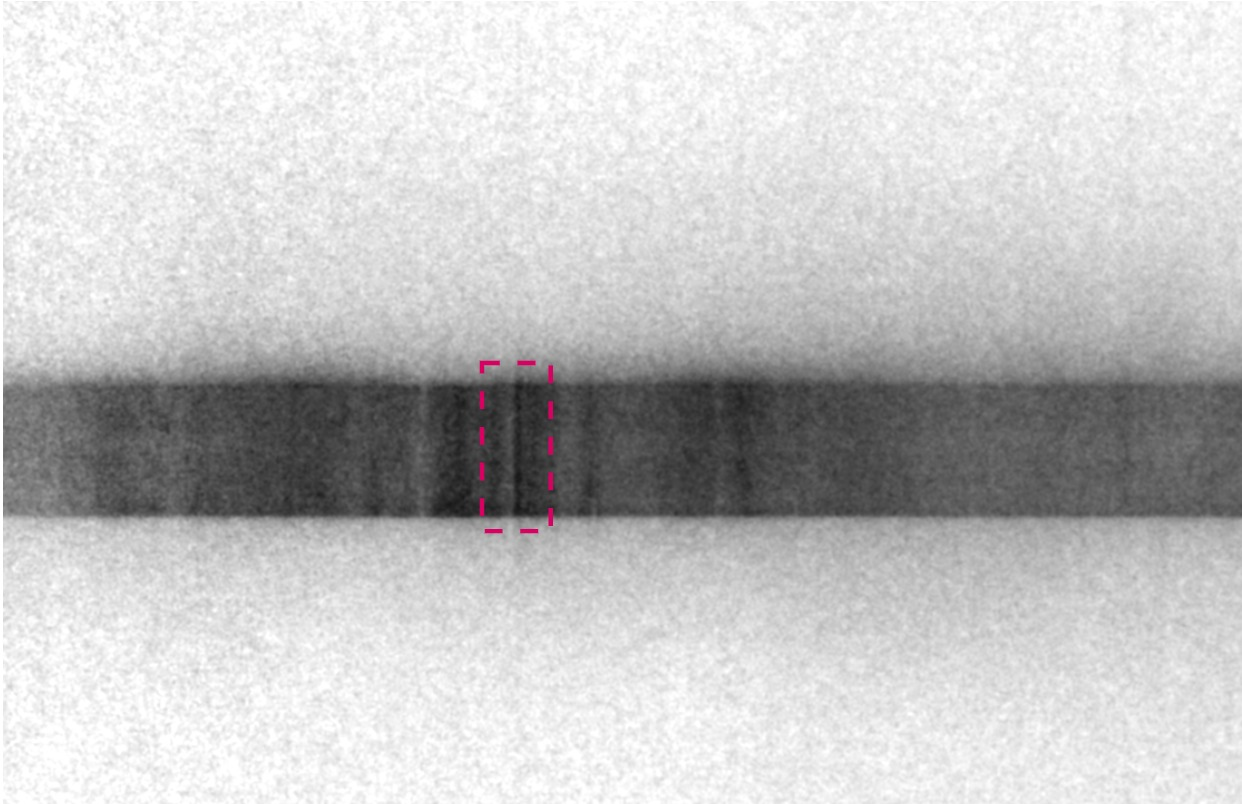
\includegraphics[width=\linewidth]{images/introduction/oxidation/layer_00010_cropped_marked}
  \caption{This oxidation spot is very likely to have on the marked region a scratch. }
\end{subfigure}
\begin{subfigure}{0.75\textwidth}
  \centering
  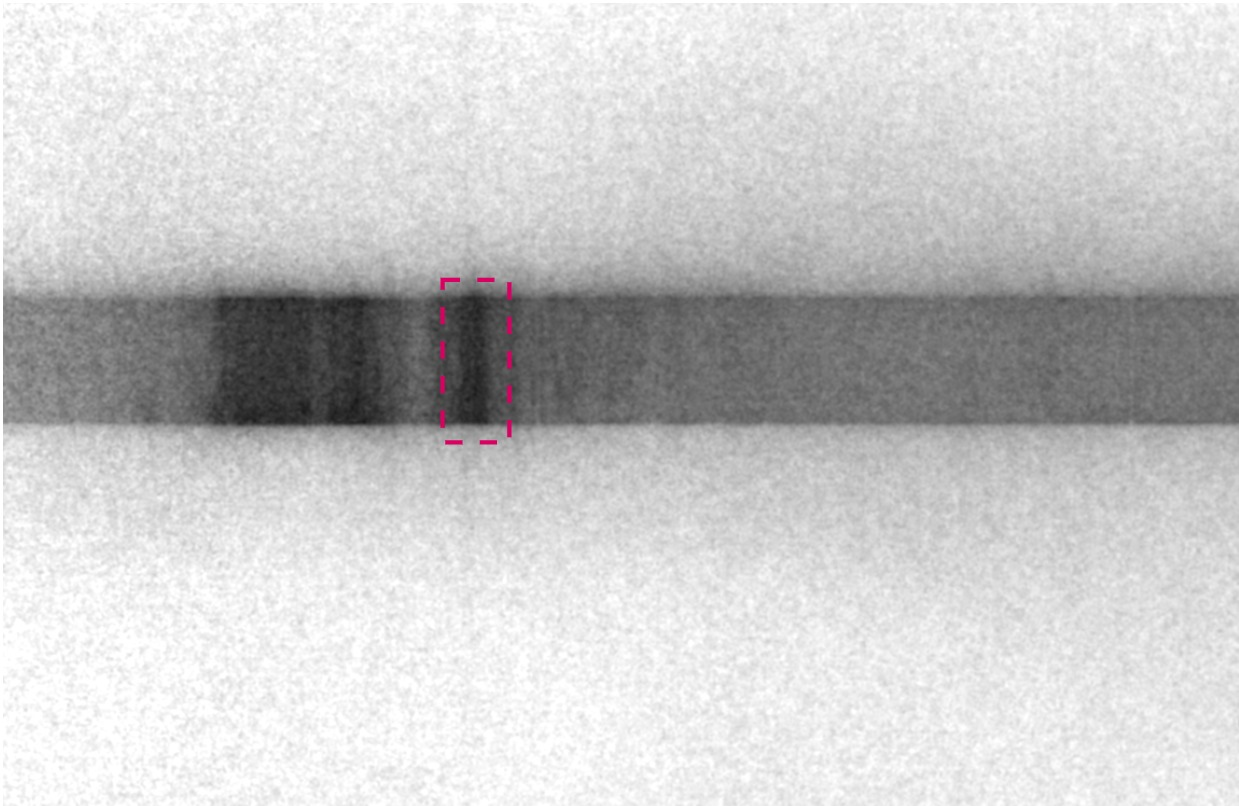
\includegraphics[width=\linewidth]{images/introduction/oxidation/layer_00016_cropped_marked}
  \caption{Harder to tell if it's a scratch or not.}
\end{subfigure}
\caption{Example of oxidation spots with potential scratches.}
\label{intro:layer_oxidation}
\end{figure}


\textbf{Choosing the neural network:}
Due to the large amount of modern neural networks, a calculated decision needed to me made. As presented in the previous section, YOLO models are currently showing a good mean average precision, despite using a single-stage approach. Another benefit of YOLO models is that the scratches can be precisely contained into a bounding box and there would be no benefit of using a model with segmentation masks. \\
There are currently a multitude of YOLO versions developed by different research groups. The final decision was to use YOLOv5 by ultralytics \cite{yolov5_git} since it quickly displayed a good performance, was written in a popular framework like PyTorch and provided support for logging and debugging tools. Other versions, such as YOLOv4 \cite{yolov4_paper}, YOLOX \cite{yolox_paper} and YOLOR \cite{yolor_paper}, were some interesting candidates, but each came with it's drawbacks. YOLOv4 had similar performance to YOLOv5, however it had longer training times and a very rudimentary logging system (no support for tools like Tensorboard). YOLOR and YOLOX had interesting twists regarding the architectures, but YOLOX used a custom framework called MegEngine \cite{megengine_git} and YOLOR lacked documentation and large community support. A few initial experiments were also not better than YOLOR or YOLOX. \\
